\documentclass{ieeeaccess}
\usepackage{cite}
\usepackage{amsmath,amssymb,amsfonts}
\usepackage{algorithmic}
\usepackage{graphicx}
\usepackage{textcomp}
\def\BibTeX{{\rm B\kern-.05em{\sc i\kern-.025em b}\kern-.08em
    T\kern-.1667em\lower.7ex\hbox{E}\kern-.125emX}}
\begin{document}
\history{Date of publication xxxx 00, 0000, date of current version xxxx 00, 0000.}
\doi{10.1109/ACCESS.2017.DOI}

\title{Preparation of Papers for IEEE ACCESS}
\author{\uppercase{First A. Author}\authorrefmark{1}, \IEEEmembership{Fellow, IEEE},
\uppercase{Second B. Author\authorrefmark{2}, and Third C. Author,
Jr}.\authorrefmark{3},
\IEEEmembership{Member, IEEE}}
\address[1]{National Institute of Standards and 
Technology, Boulder, CO 80305 USA (e-mail: author@boulder.nist.gov)}
\address[2]{Department of Physics, Colorado State University, Fort Collins, 
CO 80523 USA (e-mail: author@lamar.colostate.edu)}
\address[3]{Electrical Engineering Department, University of Colorado, Boulder, CO 
80309 USA}
\tfootnote{This paragraph of the first footnote will contain support 
information, including sponsor and financial support acknowledgment. For 
example, ``This work was supported in part by the U.S. Department of 
Commerce under Grant BS123456.''}

\markboth
{Author \headeretal: Preparation of Papers for IEEE TRANSACTIONS and JOURNALS}
{Author \headeretal: Preparation of Papers for IEEE TRANSACTIONS and JOURNALS}

\corresp{Corresponding author: First A. Author (e-mail: author@ boulder.nist.gov).}

\begin{abstract}
Abstract goes here.
\end{abstract}

\begin{keywords}
Enter key words or phrases in alphabetical 
order, separated by commas. For a list of suggested keywords, send a blank 
e-mail to keywords@ieee.org or visit \underline
{http://www.ieee.org/organizations/pubs/ani\_prod/keywrd98.txt}
\end{keywords}

\titlepgskip=-15pt

\maketitle

\section{Introduction}
\label{intro}
\PARstart{D}{ata} and Information modeling in the healthcare domain have witnessed significant improvements in the last decade owing to advances in the development of state-of-the-art Information and Communication Technologies (ICT) and formalization of storage and messaging standards. Subsequently, the scope of Healthcare Management Information Systems (HMIS), medical ontologies, and Clinical Decision Support Systems (CDSS) has broadened, beyond the operational capabilities of traditional rule based systems. One of the major reasons behind this limitation is due to the numerous heterogeneities in healthcare at data, knowledge, and process level. Thus, healthcare interoperability which aims to provide a solution to this problem, can be compartmentalized into data interoperability, process interoperability, and knowledge interoperability. Various abbreviations, used in this manuscript are listed in Table \ref{tab:abbreviations}.

\begin{table}[]
	\centering
	\caption{Abbreviations}
	\label{tab:abbreviations}
	\begin{tabular}{ll}
		\hline
		Abbreviations              & Full Form                                               \\ \hline
		ICT                        & Information and Communication Technologies              \\
		HMIS                       & Healthcare Management Information Systems               \\
		CDSS                       & Clinical Decision Support Systems                       \\
		HL7                        & Health Level Seven International                        \\
		HIMSS                      & Healthcare Information and Management Systems Society   \\
		FHIR                       & Fast Healthcare Interoperability Resources              \\
		Snomed-CT                  & Systematized Nomenclature of Medicine—Clinical Terms    \\
		LOINC                      & Logical Observation Identifiers Names and Codes         \\
		MLM                        & Medical Logic Module                                    \\
		CIMI                       & Clinical Information Modeling Initiative                \\
		UHP                        & Ubiquitous Health Platform                              \\
		NLP                        & Natural Language Processing                             \\
		BERT                       & Bidirectional Encoder Representations from Transformers \\
		UMLS                       & Unified Medical Language System                         \\
		EMR 					   & Electronic Medical Records                              \\
		EHR						   & Electronic Health Records                               \\
		MCC                        & Matthews Correlation coefficient                        \\
		NLI                        & Natural Language Inference                              \\ \hline
	\end{tabular}
\end{table}


Data interoperability resolves the heterogeneity between data artificats, to enable, seamless and interpretable communcation among source and target organizations, while preserving the data's original intention during storage, communication, and usage (as defined by IEEE 610.12 \cite{geraci1991ieee}, Health Level Seven International (HL7), and Healthcare Information and Management Systems Society HIMSS \cite{Himss_url2013}).
On the other hand, process interoperability regulates the communication among organizational processes to provide compatability between process artifacts within and seamless transformations across different organizations\cite{khan2013process}. Lastly, knowledge interoperability provides a sharing mechanism for reusing interpretable medical knowledge, acquired through expert intervention and other mechanisms, across decision support systems \cite{ali2017multi}.
In more tangible terms, healthcare interoperability at data, process, and knowledge level can be exemplified within the healthcare constraints experienced due to the emergence of Covid 19. The operational capabilities of the current healthcare service delivery infrastructure has gone under tremendous stress due to Covid 19. World over, large primary healthcare units have managed to create separate units for managing patients, suffering from extreme cases of the novel coronavirus. For secondary and tertiary care units, government involvement has become necessary to filter coronavirus patients and adhering to a national pandemic response policy. 
These complex circumstances have enhanced the need for sharing patient data and state-of-the-art medical knowledge in real-time, to provide the medical experts with a tool to make accurate and timely decisions.
Data interoperability can enable the front line medical workers to fetch, understand, and use patient data, especially comorbidities, across organizational and physical boundaries, without suffering from societal taboos that may prevent the patient from sharing their complete and accurate medical histories. Knowledge interoperability can improve the knowledge acquisition and sharing protocols to provide the medical experts such as epidieomologists and vaccinologist, with latest information on affected population trends, disease diagnosis, treatment, and followup procedures, and interpretable decisions leading to positive or negative outcomes. Process interoperability can help reduce and in some cases remove the operational redundancies between health centers. In this way, successive healthcare treatments can take benefit from earlier diagnosis, treatment, and followup procedures, thereby reducing the stress on healthcare experts and systems.
Standards such as HL7 - Fast Healthcare Interoperability Resources (FHIR), and openEHR provide the foundations for storing and communicating medical data, through the use of well defined protocols. While Systematized Nomenclature of Medicine—Clinical Terms (Snomed-CT) \cite{snomedct_url} and Logical Observation Identifiers Names and Codes (LOINC) \cite{loinc} provide a standard definition for clinical terminologies and laboratory tests, respectively. Similarly Medical Logic Module (MLM) provides a standardized way for expressing medical knowledge. However, the plethora of standards, necessitates the creation of bridging standards, that can resolve the heterogeniety between the medical standards. Substantial effort has gone into this endeavor with the Clinical Information Modeling Initiative (CIMI) \cite{CIMI2015} taking the lead in bridging the gap between HL7v3 and openEHR. Similarly, SNOMED CT and LOINC are working to resolve the redundancies between the two terminological standards since 2013. This healthcare interoperability solution follows a formal, albiet long process, which is greatly dependent on the human factor. However, the current healthcare scenario, requires a quick solution to create a scaffolding of an interoperable bridge between various healthcare providers. It is also important to ensure that this scaffolding should be able to support the formal standardization processes of the future. In \cite{Satti2020}we have presented the Ubiquitous Health Platform (UHP), which provides semantic reconciliation-on-read based data curation for resolving data interoperability between various schema. This methodology is based on the creation and management of schema maps, that can provide the framework for transforming a source schema into a target schema. 
In the current manuscript, we will present our research work to build and manage the schema map knowledge base. Overall, our methodology is based on the creation, evaluation, and application of a novel schema matching technique to identify the relationships between attributes of the participating medical data schema. These will be presented in detail, with following flow:

\begin{itemize}
	\item[$-$] Section \ref{methodology} contains the details of our methodology
	\item[$-$] Section \ref{experimentalSetup} provides the experimental setup
	\item[$-$] Section \ref{results} presents the results
	\item[$-$] Section \ref{relatedwork} presents the related work
	\item[$-$] Section 6 concludes the paper.
\end{itemize}



\section{Related Work}
\label{relatedwork}
Althubait et al. \cite{althubaiti2020combining} proposed an ontology expansion methodology that identifies and extracts new class from text articles using word embedding and machine learning techniques. The authors identified the similarity of tokens and phrases of the text articles with the exiting classes of the ontology. The target ontology is expanded with classes from text articles having greater similarity with that of already added classes. A similar word embedding technique was also used by Nozaki et al. \cite{nozaki2019semantic}, where the authors used instance based schema matching technique to identify the semantic similarity between two instances. The results of the study showed the possibility of detecting similar string attributes of different schemas. Yousfi et al. \cite{yousfi2020xmatcher} also utilized semantic base techniques and proposed xMatcher XML schemas matching approach. xMatcher transforms schemas into a set of words, followed by measuring words context, and relatedness score using WordNet. The terms from different schemas having similarities greater or equal to 0.8 are considered similar. 
Bylygin et al. \cite{bulygin2018combining} devised an ontology and schema matching approach by combining lexical and semantic similarity with machine learning approaches.  The authors used lexical and semantic measures as features and trained various machine learning algorithms including Naive Bayes, logistic regression, and gradient boosted tree. The result achieved showed that the combination of algorithms outperformed the single modal.

Martono et al. \cite{martono2017review} provided overview of previous studies related to linguistic approaches used for schema matching. Linguistic methods focused on finding strings and evaluate there similarity in different schemas. The string are normally normalized before to align both the strings before similarity comparison. The normalized strings are categories based on the information relatedness and element with similar category are compared using various similarity measure including  Jaro-distance, Lavenstein (edit-distance), and many more. Alwan et al. \cite{alwan2017survey} have summarized the techniques used in the literature for schemas and instances based schema matching. The information used for schema matching is categories into  schema information, instance and auxiliary information. Most of the searchers have used syntactic techniques (including n-gram, and regular expression), semantic techniques (including Latent Semantic Analysis, WordNet/Thesaurus and Google Similarity) for schema level and instance level matching to achieve the final goal of data/information interoperability.  Kersloot et al. \cite{kersloot2020natural} performed a comprehensive systematic review to evaluate Natural Language Processing (NLP) algorithms used for clinical text mapping onto ontological concepts. The findings of the studies were evaluated with respect to five categories; use of NLP algorithms, data used, validation and evaluation performed, result presentation, and generalization of results. The authors revealed that over one-fourth of the NLP algorithms used were not evaluated and have no validation. The systems that claimed generalization, were self evaluated and having no external validation.  

Xu et al. \cite{xu2003discovering} presented a framework for discovering indirect links besides direct links among schema elements. The indirect matches were detected for relations such as union, composition, decomposition, selection, and boolean. The indirect links are useful to handle concepts merge, split, generalization, and specialization. The matching techniques utilized in the study considered terminological relationships (word synonym and hypernym), structural characteristics, data-value characteristics, and expected data values. The experimental results revealed framework effectiveness by achieving more than 90\% precision and recall for direct and indirect link matching. 

A comprehensive survey from 176 experts including physicians and nurses was conducted by Moll et al. \cite{moll2020oncology} to check their perspectives regarding Patient Accessible Electronic Health Record (PAEHR). The authors discovered that the PAEHR positively effect after six years of operations despite negative expectations. The primary concerns revealed was logger meeting time, change in documentation practices, and increasing varies of patients regarding their health conditions. However, attitude of both healthcare service providers and patients are changing positively with respect to PAEHR and its benefits. 
 

\section{Methodology}
\label{methodology}
Healthcare interoperability, with a focus on non-standard compliant medical schema, is dependent on the generation and validation of schema maps, as discussed above. To this end, the creation of a cohesive workflow is of utmost importance. In our earlier work \cite{Satti2020} we used maximum sequence identification and suffix tress based matching for syntactic matching of two distinct data schemas. This was followed by semantic concept enrichment and subsequently concept matching, for creating rules in the form of schema maps. The simplified mapping functions, thereby created, provided a simple methodology for converting semi-structured medical data, into an interpretable, model form.
In our current methodology we have utilized state-of-the-art natural language processing (NLP) techniques to extract the schema mapping rules from semi-structured data schemas. This methodology is based on identifying similarity between vector representations of two attributes, belonging to different medical schemas. 
\textbf{Traditional NLP techniques such as WordNet are able to convert a word into an embedded vector, while Bidirectional Encoder Representations from Transformers (BERT) extracts an embedded vector from a sentence.} However, the terms forming the attribute names are bigger than a word (combination of multiple words) and smaller than a sentence. In order to resolve this problem, we extracted the set of suffixes from the terms forming the attribute names. The bidirectional nature of BERT, allows the creation of contextual embedded vectors, where each target word is affected by its neighboring words. Hence to convert the set of suffixes into a sentence, we collected the set of concepts corresponding to each suffix, from Unified Medical Language System (UMLS). This operation has two effects, firstly it is used to remove any suffix, which does not have a corresponding concept and secondly the extracted concepts are used to add context to each suffix and produce a contextual sentence. 
The following subsections provide the practical details for our methodology, from schema acquisition, to attribute name expansion, and finally schema map generation.

\subsection{Schema acquisition}
\label{schema_acq}
In the first step of our semantic reconciliation methodology, we simulate medical data acquisition from five distinct Electronic Medical Records (EMR) storage systems ($S$). These include patient reports from OpenEMR ($s_1$), 100,000 patient records from EMRBOTS ($s_2$) \cite{kartoun2016methodology}, custom database design by Pan et. al($s_3$) for supporting regional clinics and health care centers in China \cite{pan2016design}, clinical knowledge discovery tool MedTAKMI-CDI ($s_4$) \cite{inokuchi2007medtakmi}, and our custom implementation ($s_5$). Each of these medical systems as shown in \ref{fig:schema}, follows the relational database design, with logical entities, such as demographics, diagnosis, medicine or others, placed into tables which can be further linked to one or more tables. While the database design implemented by each of these systems, fulfills the need of their respective information processing applications, the lack of interoperability, in terms of identifying similar attributes or exchanging the medical data is very much evident here. 

\begin{figure*}[t!]
	\centering
	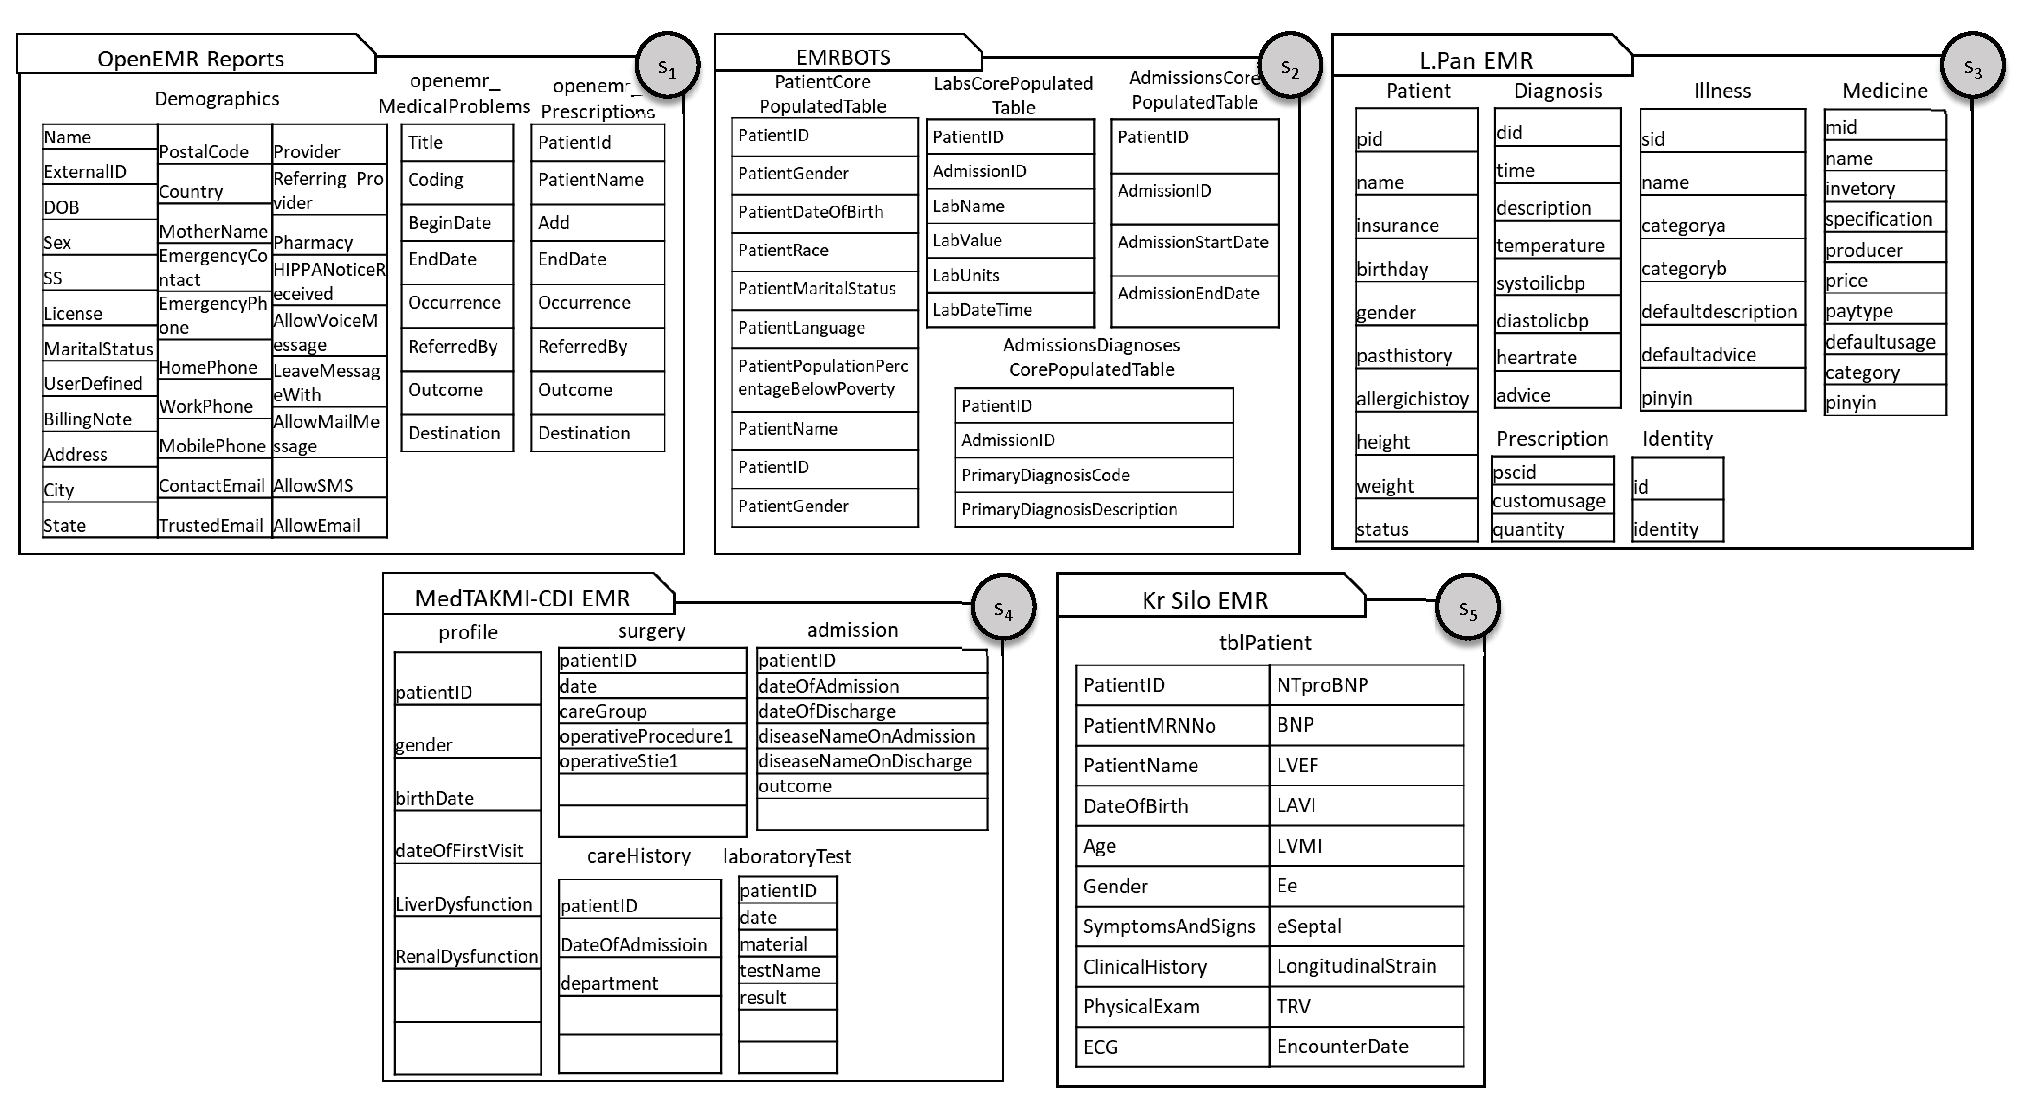
\includegraphics[scale=0.53]{schemas}
	\caption{The five medical schemas used for achieving data interoperability.}
	\label{fig:schema}
\end{figure*}

A similar notion of data heterogeneity, in terms of medical data schema, is evident across the healthcare domain. This is caused by various factors, including the lack of one all-encompassing, and universally applicable terminological standard and different normalization level for representing attributes.\\
In the former case, while SNOMED-CT provides a mechanism for identifying the standard codes for clinical terms and LOINC can be used for laboratory related terms, most attribute names are created based on the gut feeling of the database designer. Additionally, while these codes can be used to represent data instances, the data schema, achieves no benefit from the same.  Consider the terms ``name" and ``patientName", which refer to the same attribute of the patient entity.  However, since there is no standard way to represent this attribute, both are considered correct ($s_1$ and $s_3$ use the former representation, while $s_2$ and $s_5$ use the latter).\\
In the later case, differences in normalization cause semantic differences, due to which some data could be available in one schema but absent in others, such as OpenEMR demographics identifying the patient's residential location using specific attributes like ``Address", ``City", ``State", ``Postal Code", ``Country", and others. Similarly, ``EncounterDate" from $s_5$ is semantically similar to ``BeginDate" of ``openemr\_MedicalProblems" table in $s_1$, ``AdmissionStartDate" of ``LabsCorePopulatedTable" in $s_2$, 
``time" in ``Diagnosis" table of $s_3$, and  ``dateOfAdmission" in ``Diagnosis" and ``CareHistory" tables of $s_4$.
Finally, $s_1$ and $s_3$ have separate tables containing the medicinal prescription details, however the same details are unavailable in $s_2$, $s_4$, $s_5$. Once again, this is not an incorrect behavior since this information, might not be a part of the context or the requirements for the EMR/EHR storage systems.
In fact, the change in context of the medical data storage system from the initial time of development to a later stage of collaborative processing systems, is the main cause of heterogeneity. In order to provide an interoperable solution, it is therefore necessary to enhance the semantics of each data attribute by its contextually equivalent sentence. 

\subsection{From Attribute to Sentence}
\label{schema_prepro}
In order to process the EMR/EHR schema set $S$ and produce a set of corresponding semantically enriched sentences, we use the data representation $s_i$, generated through the process explained in sequence acquisition to collect the various medical fragments in memory. We then iterate over these fragments, building a set of attributes, distinguished by their name, schema's name, table's name, schema's version, source, and recorded data. This entails that ``PatientID" from each of the four tables in $s_2$, and ``patientID" from five tables in $s_4$, would result into nine attributes (assuming, as in the current case, of no differences in versions of these systems).
For each attribute, we then generate the suffix array, which provides all possible substring representations contained within the attribute name. In order to generate the set of suffixes, we employ three strategies, forward suffix generation, whereby for a word $w$ of length $n$, $n-1$ suffixes of size 2 to $n-1$ are produced, backward suffix generation, to produce $n-1$ suffixes in reverse order with size $n-1$ to 2, and regular expression based suffix generation, which splits each word on, change of case, special characters(such as -, \_, !, and others), and numbers. In this way a large list of suffixes is generated, which is combined using a ``TreeSet" data structure of Java, which internally sorts this list as well. An example of this suffix generation process, using the attribute name ``dateOfAdmission" as it appears in $s_4$ is shown in \ref{fig:suffix_attribute}.


\begin{figure*}[t!]
	\centering
	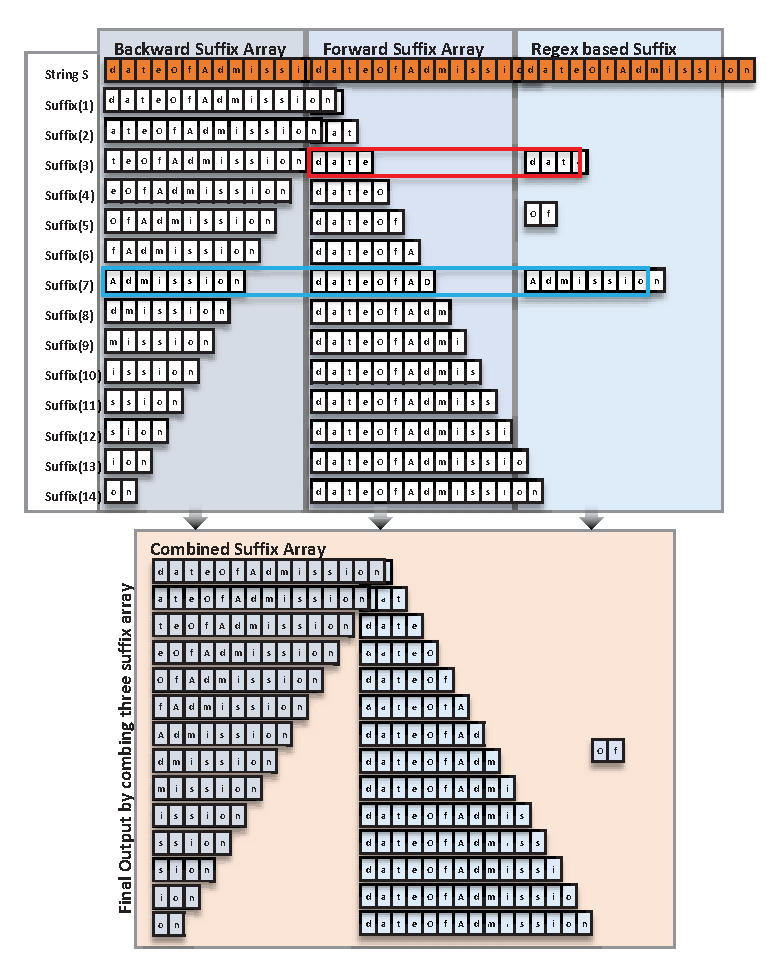
\includegraphics[scale=0.53]{suffixAttribute}
	\caption{Suffix attributes.}
	\label{fig:suffix_attribute}
\end{figure*}

Suffix strings for similar attributes such as ``AdmissionStartDate". ``diseaseNameOnAdmission", and ``AdmissionEndDate" appear in $s_2$, produce many, synctactically similar suffixes, to the presented example. This process, is only able to generate syntactic suffixes, producing many incoherent and unrelated suffixes. In order to counter this problem, and to limit the list of suffixes within the domain, we then query UMLS, with exact search strategy, looking for the existence of any concepts, against each suffix. In case, no semantic concept is found for a particular suffix, it is removed from the final Suffix Array. On the other hand, if atleast one semantic concept is found against the queried suffix, it is retained. Meanwhile the process continues for the next attribute, then the next table, and finally the next system, till no further processing is possible. 
The set of suffixes and their corresponding concepts are then used to build the sentence, where by each concept, corresponding to a suffix is appended next to the suffix. An example of the resultant sentence for the attribute ``DateOfAdmission" is shown as follows:\\

\framebox{\parbox{\dimexpr\linewidth-2\fboxsep-2\fboxrule}{\itshape%
		
		``Date Value type - Date date allergenic extract Date in time Data types - Date Date Fruit;Of SPI1 wt Allele SPI1 gene TAF1 wt Allele BRIP1 gene Within Degrees fahrenheit Oral contraception BRIP1 wt Allele;Da Displacement of abomasum dalton Anterior descending branch of left coronary artery deca units cytarabine/daunorubicin protocol Dai Chinese Asymptomatic diagnosis of Drug Accountability Domain;ion Iontophoresis Route of Drug Administration Ions;on SPARC wt Allele Osteonectin SPARC gene On (qualifier value) Upon - dosing instruction fragment;Admission Admission activity Hospital admission;Dat SLC6A3 gene SLC6A3 wt Allele dopamine transporter Direct Coombs test SLC6A3 protein, human Test Date cytarabine/daunorubicin/thioguanine Alzheimer's Disease;mission Religious Missions;"
}}\\

Here the various suffixes and their concepts are seperated by the symbol ``;", however together they form one sentence, for which an embedded vector is generated. 

\subsection{Schema Map generation}
\label{schema_map_gen}

Schema Maps, provide an interoperable bridge between two medical systems ($s_i \wedge s_j$), by identifying the semantic relationship between their participating attributes. This identification is based on the similarity between the embedded vectors, of the semantically enriched sentences, corresponding to each data attribute. While the embedded vectors can be generated using any methodology (we tested 11 methodologies, with WordNet and 10 models based on BERT (including BERT base, BERT large, distilBert, and RoBERTa) further detailed in section \ref{experimentalSetup}), the large/STSb version of RoBERTa\cite{reimers-2019-sentence-bert},provides the best results. The pair of embedded vectors thus produced are then used to calculate cosine similarity, which is based on the inverse cosine distance between them. For our classification, we used the raw results (unnormalized) of cosine similarity, which produces a score between -1, and 1. Cosine similarity score of 0 indicates orthogonal relationship between the two vectors, which in our scenario indicates that the two sentences, and by extension their attributes are not related to each other. -1 indicates, inverse relationship between the attributes, while 1 indicates the two attributes are very much the same.
For producing our schema maps, we are interested in three types of relationships, ``equal" (the two attributes are same), ``related" (the two attributes are related to each other), and ``unrelated" (no relationship between the attributes). In order to classify the similarity results, into one of these three classes, we then calculated the best thresholds, using Matthews Correlation coefficient (MCC) \cite{chicco2020advantages} for classifying each instance as ``equal", ``related", and ``unrelated". Finally on a test dataset we evaluated our multi-class classification approach, to identify the relationships between each pair of attributes.



\section{Experimental Setup}
\label{experimentalSetup}
In our earlier work \cite{Satti2020} $s_1$, $s_2$, and $s_5$ were used to generate over 115 million patient records, which are converted into a semi-structured form and stored in Hadoop Distributed File System (HDFS). We extended the same setup to create an additional 100,000 records, for 1000 patients with 3 medical fragments for $s_1$, $s_2$, and $s_4$, and 97 randomly selected and generated medical fragments amongst $s_1$, $s_2$, $s_3$, $s_4$ and $s_5$. These fragments, follow various design elements, supporting a variety of valid relational storage architectures. Such as, $s_1$, $s_2$ and $s_4$ are represented by creating a separate medical fragment for each participating table, $s_3$ utilizes its medical fragment to generate a linked record (from a linked object graph), where by the attributes can refer to other objects besides the elements of $t$, mimicking the application of explicit foreign keys, and $s_5$ is a flat table structure. The code to generate this data set is available at ``uhp\_map\_generation"\footnote{https://github.com/desertzebra/UHP\_v4/tree/main/uhpr\_storage}. This application produces three custom formatted files, containing an index for patients, an index for their medical fragments, and the medical fragment, corresponding to the EMR data. Using the medical fragments file, we then generate the semantically enriched attribute \footnote{https://github.com/desertzebra/UHP\_v4/tree/main/uhp\_map\_generation}, which contains the suffixes and their concepts corresponding to each EMR data attribute. The resulting set of enriched attributes are temporarily stored in a ``json" file, which is then read by the same application to partially generate the schema maps. This process, is used to create 20,349 distinct pairs of attributes, across $s$. Each pair also contains the ``relationshipList", which stores the results of fuzzy string matching\cite{FuzzyWuzzy} \footnote{Java Library: https://github.com/xdrop/fuzzywuzzy} between the attribute names. 
The ``json" file thus produced, is then used by a python script to generate the semantically enriched sentences and their embedded vectors using Word2Vec, and 10 pre-trained BERT NLI models \cite{reimers-2019-sentence-bert}. The BERT models include 'bert-base-nli-stsb-mean-tokens', 'bert-large-nli-stsb-mean-tokens', 'roberta-base-nli-stsb-mean-tokens', 'roberta-large-nli-stsb-mean-tokens', 'distilbert-base-nli-stsb-mean-tokens', 'bert-base-nli-mean-tokens', 'bert-large-nli-mean-tokens', 'roberta-base-nli-mean-tokens', 'roberta-large-nli-mean-tokens', and 'distilbert-base-nli-mean-tokens'. 
The embedding vectors are then compared using cosine similarity, which produces a score between -1 and 1.
The rationale behind switching the applications at various stages, is to cache the results and create checkpoints for restarting any failed stages, easily. Additionally, since python provides better support for easy generation of embedding vectors, it was thus preferred over the Java based implementation, which is otherwise very beneficial for other tools. These applications were executed on a workstation running Ubuntu 20.04.2 on top of AMD Ryzen 3 2200G, and 32GB ram.

\section{Results}
\label{results}

The validity of our proposed approach has been evaluated using several techniques, including comparison of the proposed semantic matching process with fuzzy string matching, embedded vector generation and comparison using Word2Vec, and 10 BERT nli models. 

\subsection{Dataset Annotation}
In order to compare our computed models with ground truth, and to identify the best thresholds for classifying each instance as ``equal", ``related", or ``unrelated" 4 human annotators were utilized, to anonymously, score the similarity of each pair of attribute names. In order to support this process, we first repurposed one of our generated data matrix, by marking all attribute pairs belonging to the same schema with the symbol ``-". Following this, the annotators, marked each cell corresponding to a pair of attributes (conversely, each attribute pair corresponds to two cells, with the positioning of the pair-participants swapped; which is used for clarity and identify correct relationships between the attribute on left and attribute on right), by determining the similarity in terms of dissimilar as ``0", exactly similar as ``1", row attribute as child of column attribute as ``<", row attribute as a parent of the column attribute as ``>", and finally, unknown as ``~". The data sheets generated after this extensive human effort, have been made available for other researchers\footnote{https://github.com/desertzebra/EMR-Interoperability/tree/master/Implemenation/Data/Annotated}.

\begin{figure*}[t!]
	\centering
	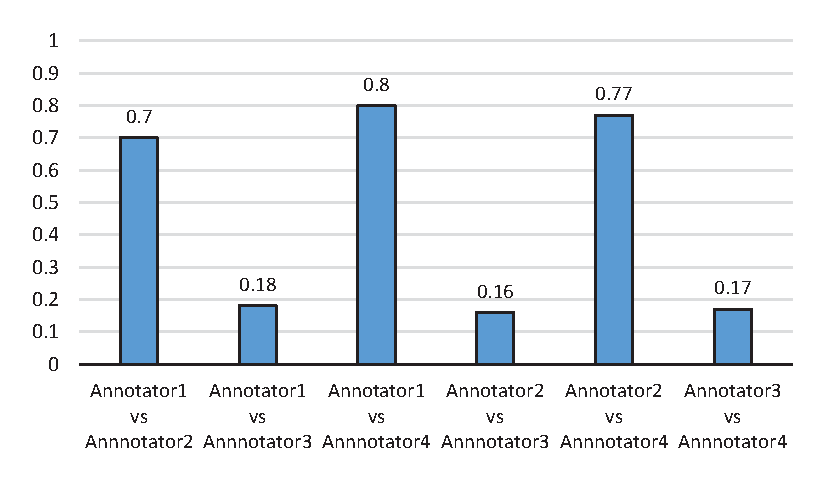
\includegraphics{kappaInterAnnotatorAgrement}
	\caption{Cohen's Kappa (d) score between the four annotators}
	\label{fig:kappaInterAnnotatorAgrement}
\end{figure*}

These sheets, additionally contain some missing values, which were left out by the annotators, but in order to maintain their originality, these values were not filled; instead during our evaluation for these datasets, the missing values were considered as having the score ``0". Using \textbf{Cohen's Kappa score (d)}, we evaluated the inter-rater agreement of these annotations, which have been visualized in Figure \ref{fig:kappaInterAnnotatorAgrement}. It can be seen in this plot, that ``Annotator3" has very small correlation with the other 3 annotators. This difference can be traced back to the number and type of annotations performed by each annotator, which is shown in Table \ref{tab:annotator_marking}. The ``Annotator3" has marked 2103 cells as related (one of >, < , or ~) and left 153 as empty. However, even in the presence of these difference, it is pertinent to include the data for all annotators in order to avoid any biasedness. 

\begin{table*}
	\centering
	\caption{Annotations performed by the four annotators on five medical schema}
	\label{tab:annotator_marking}
	\begin{tabular}{|l|l|l|l|l|l|}
		\hline
		Method     & Total Matches & Marked as Equal & Marked as Related & Marked as Unrelated & Not Marked \\ \hline
		Annotator1 & 40698         & 238             & 109               & 40351               & 0          \\
		Annotator2 & 40698         & 241             & 116               & 40341               & 0          \\
		Annotator3 & 40698         & 260             & 2103              & 38182               & 153        \\
		Annotator4 & 40698         & 225             & 62                & 40400               & 11         \\ \hline
	\end{tabular}
\end{table*}


This annotated data was then processed, to replace all related entries with ``0.5" and all``-" with ``0", while the values for similar at ``1" and ``0" for dissimilar were kept the same. This conversion was then used to produce a consolidated dataset of 40,698 attribute pairs, using mode scores of all annotators, for each cell. We also tested average scores between the annotators, but that would produce scores between ``0", ``0.5", and ``1", greatly increasing the number of classes for classification. Hence the maximum agreement between the annotators, maintains the final label values within these three classes, which become easier to evaluate. Additionally, the original dataset and its mode consolidated form is biased in favour of class "0", since most attribute pairs are not related to each other.
This dataset is then split into development and testing partitions with a ratio of 70:30. The development partition is used for threshold selection, based on the best MCC score for identifying class ``equal", followed by best scores for class ``related" and finally best of class "unrelated". The optimal threshold thus achieved is used to classify the instances of the test dataset, which is finally evaluated on its MCC and F-1 score.

\subsection{Threshold Selection}
A good text classification methodology is dependent on the correct choice of a threshold, which can maximize the target class participation. In case of independent labels, area under the precision recall curve can provide this optimal measure, however as in our case, for dependent classes on a biased dataset the Matthews Correlation Coefficient (MCC), is better\cite{chicco2020advantages}. Since our aim is to apply an optimal text similarity classifier to resolve this multi-class problem (class 0, class 0.5, and class 1), we have to test various threshold scores for separating the instances between 0 and 0.5 ($t_1$), and then 0.5 and 1($t_2$). Additionally, since our aim is to correctly identify the similar attribute instances, it is pertinent to maximize the classification performance of class 1 (similar), followed by class 0.5 (related), and finally class 0 (unrelated).
With a step size of 0.05 ($step_size$), and starting from $t_1$ as 0.0 and $t_2$ as $t_1$ + $step_size$, we move the thresholds until $t_2$ reaches 1, followed by increase in $t_1$ by step size. Eventually, $t_1$, reaches 0.95 and $t_2$ reaches 1, at which point, the process stops. This is to ensure that $t_1$ remains behind $t_2$, for all iterations, measuring MCC score, for the 12 models. These models include, ``Fuzzy\_Wuzzy", ``Word2Vec", and 10 BERT based models.

\begin{figure*}[t!]
	\centering
	\includegraphics[scale=0.83]{thresholdSelection}
	\caption{Thresholds selection.}
	\label{fig:thresholdSelection}
\end{figure*}
Threshold values for Word2Vec are placed at the lower end of the spectrum, indicating a very large number of instances are classified as similar (above similarity score of 0.1), while a small number of instances (with similarity score 0.05) are classified as dissimilar. Similarly, the class related lies within the similarity threshold of 0.05 similarity points. It can be observed that the threshold for selecting the related class, is within 0.05 points, in all except one case (bert-large-nli-mean-tokens where the difference is 0.15 points). Five BERT based models, trained on the STSb dataset, all have minimum threshold values of 0.85 and maximum of 0.9, while the 4 remaining BERT models, lie between 0.9 and 0.95. These results show a general trend, of how the cosine similarity varies/maintains itself, against embedded vectors generated from various pre-trained models. In absolute terms, however these threshold values provide the mechanism for classifying the test dataset, which is evaluated for performance, in the next subsection.

\subsection{Model Evaluation}
On unseen test dataset, with thresholds selected in the previous step and the 12 models, we measured the performance score, using one vs all binarization of the multi-class classification and overall as well. 
In the first case, we evaluated 






Finally, we evaluated the 


The results of fuzzy string comparison ($D_f$) on the attribute names of each pair, can be visualized using the heatmap shown in \textbf{figFuzzyWuzzy}. Similarly, the results of comparison using BERT based word embedding of the attribute names ($D_b$), is shown in \textbf{figBase}. Finally, the heatmap of the syntactic and semantic matching of the AA's using our proposed Algorithm \ref{knowledgeEvolAlgo} ($D_p$), is shown in \textbf{figSynAndSemMatching}. The values, for each cell range between ``0" and ``1", with higher values indicating a larger match between the elements, in each of these cases. The black areas of these heatmaps, indicate missing values, while white indicates a matching value of ``0". The few areas with red color, indicate the values above ``0.9", while blue areas indicate values above ``0.8". 


Overall, the number of similarities above the threshold values of ``0.8" are greatly increased from $D_f$, to $D_b$, and then to $D_p$ (proposed methodology). Changing the threshold value in $D_p$ to ``0.9", brings it relatively closer to $D_b$. This is due to our proposed similarity matching methodology, which gives an equal score (0.5) to the values obtained from both syntactic and semantic matches. Since the decision made at the syntactic evaluation is binary (0 or 1), thus for a similarity score of ``0.8", in $D_p$, ``0.5" represents the syntactic similarity, and ``0.3" semantic similarity. The semantic similarity value, obtained from this rescaling process, would in turn represent an original value of ``0.6" from $D_b$. Therefore, for an equal semantic representation, the value of semantic similarity after rescaling (between 0 and 0.5) should be ``0.4", and originally ``0.8". \textbf{figSynAndSemMatching0.9} shows the heatmap, of similarity matrix, obtained from $D_p$ with the threshold values as ``0.9".

Generally, a comparison of these heatmaps, indicate an increase in the recall rate of the methodology. This is due to the fact, that our proposed methodology is able to match a larger number of AAs, providing 50\% of the score to the syntactic match, thereby increasing the count of cells without a missing value. This approach is also able to reduce the impact of semantic matching from names, which might contain repeated words, such as ``patient" but in reality refer to disparate concepts, such as ``PatientName" and "PatientDateOfBirth". Another important aspect of our matching process is the inclusion of semantic concepts and suffixes, as a sentence before its conversion to an embedded vector. As discussed earlier, this process is used to reduce the impact of syntactic matches alone, which would give a higher score to the attributes ``PatientName" and ``PatientGender", which refer to different concepts. The inclusion of concepts behind ``Name" and ``Gender" part of these names, allow for an improved comparison. 


In order to evaluate the accuracy and precision rates of these methodologies, we then compared the results of our computed methods $D_f$, $D_b$, and $D_p$, with the average scored datasets by the human annotators. A visualization of the resultant Cohen's Kappa score for the 261 participating attributes, is shown in \textbf{figComputedComparisonKappaScore}. The bar chart shown in this visualization, indicates, an overall greater positive agreement between our proposed methodolody $D_p$, and the average scores of the annotators. The same is shown by the \textbf{orange} colored peaks in this dataset, which in all cases is either equivalent to the other approaches ($D_f$ and $D_b$), or better than them.

\section{Conclusion}
Conclusion goes here. 


\section*{Acknowledgment}

Acknowledgment goes here.



\bibliographystyle{unsrt}
\bibliography{references}


\begin{IEEEbiography}[{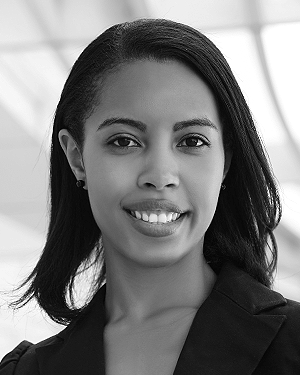
\includegraphics[width=1in,height=1.25in,clip,keepaspectratio]{a1.png}}]{First A. Author} (M'76--SM'81--F'87) and all authors may include 
biographies. Biographies are often not included in conference-related
papers. This author became a Member (M) of IEEE in 1976, a Senior
Member (SM) in 1981, and a Fellow (F) in 1987. The first paragraph may
contain a place and/or date of birth (list place, then date). Next,
the author's educational background is listed. The degrees should be
listed with type of degree in what field, which institution, city,
state, and country, and year the degree was earned. The author's major
field of study should be lower-cased. 

The second paragraph uses the pronoun of the person (he or she) and not the 
author's last name. It lists military and work experience, including summer 
and fellowship jobs. Job titles are capitalized. The current job must have a 
location; previous positions may be listed 
without one. Information concerning previous publications may be included. 
Try not to list more than three books or published articles. The format for 
listing publishers of a book within the biography is: title of book 
(publisher name, year) similar to a reference. Current and previous research 
interests end the paragraph. The third paragraph begins with the author's 
title and last name (e.g., Dr.\ Smith, Prof.\ Jones, Mr.\ Kajor, Ms.\ Hunter). 
List any memberships in professional societies other than the IEEE. Finally, 
list any awards and work for IEEE committees and publications. If a 
photograph is provided, it should be of good quality, and 
professional-looking. Following are two examples of an author's biography.
\end{IEEEbiography}

\begin{IEEEbiography}[{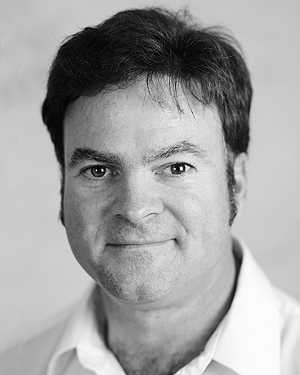
\includegraphics[width=1in,height=1.25in,clip,keepaspectratio]{a2.png}}]{Second B. Author} was born in Greenwich Village, New York, NY, USA in 
1977. He received the B.S. and M.S. degrees in aerospace engineering from 
the University of Virginia, Charlottesville, in 2001 and the Ph.D. degree in 
mechanical engineering from Drexel University, Philadelphia, PA, in 2008.

From 2001 to 2004, he was a Research Assistant with the Princeton Plasma 
Physics Laboratory. Since 2009, he has been an Assistant Professor with the 
Mechanical Engineering Department, Texas A{\&}M University, College Station. 
He is the author of three books, more than 150 articles, and more than 70 
inventions. His research interests include high-pressure and high-density 
nonthermal plasma discharge processes and applications, microscale plasma 
discharges, discharges in liquids, spectroscopic diagnostics, plasma 
propulsion, and innovation plasma applications. He is an Associate Editor of 
the journal \emph{Earth, Moon, Planets}, and holds two patents. 

Dr. Author was a recipient of the International Association of Geomagnetism 
and Aeronomy Young Scientist Award for Excellence in 2008, and the IEEE 
Electromagnetic Compatibility Society Best Symposium Paper Award in 2011. 
\end{IEEEbiography}

\begin{IEEEbiography}[{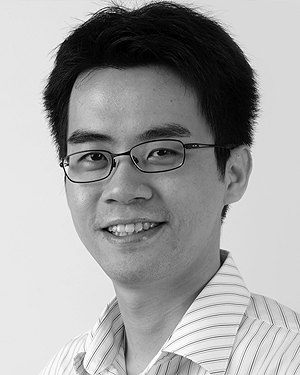
\includegraphics[width=1in,height=1.25in,clip,keepaspectratio]{a3.png}}]{Third C. Author, Jr.} (M'87) received the B.S. degree in mechanical 
engineering from National Chung Cheng University, Chiayi, Taiwan, in 2004 
and the M.S. degree in mechanical engineering from National Tsing Hua 
University, Hsinchu, Taiwan, in 2006. He is currently pursuing the Ph.D. 
degree in mechanical engineering at Texas A{\&}M University, College 
Station, TX, USA.

From 2008 to 2009, he was a Research Assistant with the Institute of 
Physics, Academia Sinica, Tapei, Taiwan. His research interest includes the 
development of surface processing and biological/medical treatment 
techniques using nonthermal atmospheric pressure plasmas, fundamental study 
of plasma sources, and fabrication of micro- or nanostructured surfaces. 

Mr. Author's awards and honors include the Frew Fellowship (Australian 
Academy of Science), the I. I. Rabi Prize (APS), the European Frequency and 
Time Forum Award, the Carl Zeiss Research Award, the William F. Meggers 
Award and the Adolph Lomb Medal (OSA).
\end{IEEEbiography}

\EOD

\end{document}
